

\begin{frame}[ctb!]
  \frametitle{Nested Components}
  \begin{figure}[h!]
    \begin{center}
      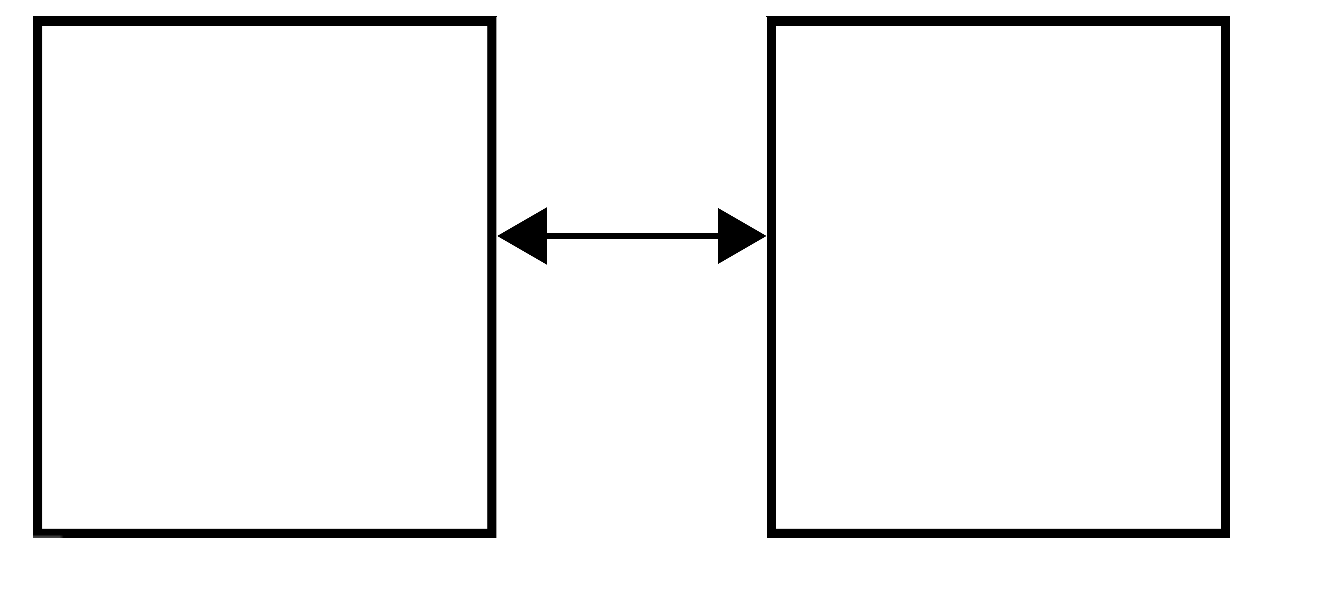
\includegraphics[width=\textwidth]{../report/chapters/paradigm/flow.eps}
    \end{center}
    \caption{The nested components supply thermal flux and concentration 
    information to each other at the boundaries.}
    \label{fig:flow}
  \end{figure}
\end{frame}



\begin{frame}[ctb!]
  \frametitle{Mixed Cell : Permeable Porous Medium}
  % Waste Form
  \begin{figure}[h!]
    \begin{center}
      \includegraphics[height=.6\textwidth]{../report/chapters/future/contaminated1.eps}
    \end{center}
  \end{figure}
\end{frame}

\begin{frame}[ctb!]
  \frametitle{Mixed Cell : Permeable Porous Medium with Degradation}
  % Waste Form
  \begin{figure}[h!]
    \begin{center}
      \includegraphics[height=.6\textwidth]{../report/chapters/future/contaminated.eps}
    \end{center}
  \end{figure}
\end{frame}

\begin{frame}
  \frametitle{Nested Components}
  \begin{itemize}
    \item Waste Form
      \begin{itemize}
        \item Mixed Cell 
        \item with Rate Based Degradation Model
        \item and solubility limits
        \item Data for various waste forms
      \end{itemize}
    \item Waste Package
      \begin{itemize}
        \item Rate Based Failure Model
        \item Data for various waste packages
      \end{itemize}
    \item Buffer
      \begin{itemize}
        \item Mixed Cell 
        \item with Rate Based Degradation Model
        \item Data for various buffers
      \end{itemize}
    \item Geology
      \begin{itemize}
        \item Solute transport model
        \item Data for various geologic media
      \end{itemize}
  \end{itemize}
\end{frame}

